%%
%% This is file `template.tex',
%% generated with the docstrip utility.
%%
%% The original source files were:
%%
%% articleingud.dtx  (with options: `tmple')
%% 
%% -------------------------------------------------------------------
%%                           LICENSE
%% -------------------------------------------------------------------
%% 
%% This is a generated file.
%% 
%% Copyright (C) 2012-2015 by Omar Salazar
%% osalazarm@correo.udistrital.edu.co
%% Laboratory for Automation and Computational Intelligence (LAMIC)
%% Engineering Department
%% Universidad Distrital Francisco Jose de Caldas
%% Bogota, Colombia
%% http://www.udistrital.edu.co/
%% 
%% This file may be distributed and/or modified under the
%% conditions of the LaTeX Project Public License, either
%% version 1.2 of this license or (at your option) any later
%% version. The latest version of this license is in:
%% http://www.latex-project.org/lppl.txt
%% and version 1.2 or later is part of all distributions of
%% LaTeX version 1999/12/01 or later.
%% 
%% This work has the LPPL maintenance status `maintained'.
%% 
%% The Current Maintainer of this work is Omar Salazar.
%% 
%% This work consists of the source files:
%%  - articleingud.dtx (documented LaTeX file)
%%  - articleingud.ins (installer)
%% 
\documentclass[letterpaper,12pt,twoside]{articleingud}
%%----------------------------------------------------------
%%                OPTIONS
%%----------------------------------------------------------
%% Use the following options in
%% \documentclass[<options>]{articleingud}
%%
%%  -- Point size:  10pt (default),
%%                  11pt,
%%                  12pt
%%  -- Paper size:  letterpaper (default),
%%                  a4paper,
%%                  a5paper,
%%                  b5paper,
%%                  legalpaper,
%%                  executivepaper
%%  -- Orientation: portrait (default)
%%                  landscape
%%  -- Print size:  oneside (default),
%%                  twoside
%%  -- Quality:     final (default),
%%                  draft
%%  -- Columns:     onecolumn (default),
%%                  twocolumn
%%  -- peer review: peerreview
%%  -- Equation numbering (equation numbers on
%%                         the right is the default):
%%                  leqno
%%  -- Displayed equations (centered is the default):
%%                  fleqn (equations start at the same
%%                         distance from the right side)
%%  -- Open bibliography style (closed is the default):
%%                  openbib
%%----------------------------------------------------------
%%           PREAMBLE
%%----------------------------------------------------------
%%
%%      Here you can load packages with \usepackage
%%      and make (re)definitions with
%%      \newcommand, \renewcommand, \newenvironment,
%%      \renewenvironment, etc, ...
%%
%%----------------- PACKAGES -------------------------------
\usepackage{amsmath}
\usepackage{amsfonts}
\usepackage{amssymb}
\usepackage{graphicx}
\usepackage[tight,footnotesize]{subfigure}
\usepackage{cite}
\usepackage{eso-pic} % For 'ingenieria' picture
\usepackage{fancybox} % For framed title and abstracts
\setlength{\fboxsep}{10pt} % Space between the rule and the contents of the box
\usepackage{siunitx}% Units physics
\usepackage{hyperref}% Add Hyperlinks
\usepackage[utf8]{inputenc} %Tildes
%%----------------- (RE)DEFINITIONS------------------------
\makeatletter
\newcommand{\INGUDAdjustbox}{% % Adjust extra space added by fancybox in Ovalbox
  \addtolength{\columnwidth}{-2\fboxsep}%
  \addtolength{\columnwidth}{-4\@wholewidth}}
\makeatother
%\renewcommand{\figurename}{Figura}
%\renewcommand{\tablename}{Tabla}
%\renewcommand{\refname}{Referencias}
%%----------------------------------------------------------
%%           DOCUMENT
%%----------------------------------------------------------
\begin{document}
%%----------------------------------------------------------
%%       PAPER'S INFORMATION
%%----------------------------------------------------------
\title
  [Short title of the paper]% (Optional)
  {PowerPAR LED photosynthesis}% (Required)
  {High power LED lighting system for the precision agriculture}% (Required)
  {Research}% (Required) Research/Review/Case-study/Short/Opinion paper
\author
  [First Author Name\and% <-- Each author should be separated with \and
   Second Author Name\and
   Last Author Name]% (Optional)
  {Diego Javier Mena Amado% <-- Do not erase this percentage symbol
   \thanks[Correspondence email: jmenaa@correo.udistrital.edu.co]
          {1}% <-- Use the same label ('a-z' or '0-9') for authors with the same affiliation
          {1st Author affiliation}\and
   Cesar Andrey Perdomo Charry% <-- Do not erase this percentage symbol
   \thanks%[Correspondence email: 2nd-author@email.org]
          {2}% <-- Affiliation label
          {2nd Author affiliation}
  \\Luis Martín Santamaria% <-- Do not erase this percentage symbol
  \thanks%[Correspondence email: last-author@email.org]
          {3}% <-- Affiliation label
          {Last Author affiliation}}% (Required)
\date
  {Received: dd-mm-yyyy.
   Modified: dd-mm-yyyy.
   Accepted: dd-mm-yyyy}% (Required)
\INGUDsetciteinfo
  {\addtolength{\columnwidth}{-1in}% Picture's width
   \addtolength{\columnwidth}{-10pt}% Space between picture and text
   
\includegraphics[width=1in]{by-nc-sa}% Picture
   \nobreak\hfill\nobreak
   \Ovalbox{\INGUDAdjustbox
   \parbox[b][][b]{\columnwidth}{\raggedright % Text
   \textcopyright{} The authors;
   licensee: Revista INGENIER\'IA. ISSN 0121-750X, E-ISSN 2344-8393.
   Cite this paper as: Author, F., Author, J., Author, S.:
   The Title of the Paper. INGENIER\'IA, Vol. XX, Num. XX, 2015 pp:pp.
   doi:10.14483/udistrital.jour.reving.20XX.X.aXX}}}% (Required)
\INGUDsetvolume
  {1}%<-- Volume (the number only)
\INGUDsetnumber
  {1}%<-- Number (the number only)
\INGUDsetinitialpage
  {1}%<-- First page of the paper (the number only)
%%----------------------------------------------------------
%%                TITLE
%%----------------------------------------------------------
\noindent
\Ovalbox{\INGUDAdjustbox
\begin{minipage}{\columnwidth}
\maketitle
\end{minipage}}
\endmaketitle
\AddToShipoutPictureFG*{% Needed to put 'ingenieria' picture
  \AtTextUpperLeft{%
    \vbox{\hbox to\columnwidth{\hfil
    
\includegraphics[height=0.5in]{ingenieria}}\vss}}}%
%%----------------------------------------------------------
%%                ABSTRACT
%%----------------------------------------------------------
%\textw
\vfil
\noindent
\Ovalbox{\INGUDAdjustbox
\begin{minipage}{\columnwidth}
\begin{abstract} % no more than 300 words is recommended
The precise control of the light to which the crops are exposed allows to improve the production and to expand the season margin of harvest season. Some aspects improved are the organoleptic properties that are usually related to high quality products, such as: their shape, pigmentation or color of plants and fruits, their smell and taste, the precocity of the crops and even a remarkable improvement in the control of pests and diseases. This research aims to expand experimental scientific and technological information, to date, on photosynthetically active radiation (PAR), known as radiation integrated by ranges of wavelengths that are capable of producing photosynthetic activity in plants and other organisms, such as microalgae and bacteria. This article shows the experimental development of a wireless system for the monitoring, control and programming of color composition in artificial light capable of stimulating the photosynthetic reaction in plants, as a tool to improve the efficiency in horticultural production and for the investigation of photometric effects in photosynthetic organisms, implementing high power LED technologies.
\end{abstract}
\end{minipage}}
%%----------------------------------------------------------
%%                RESUMEN
%%----------------------------------------------------------
\renewcommand{\abstractname}{Resumen}
\vfil
\noindent
\Ovalbox{\INGUDAdjustbox
\begin{minipage}{\columnwidth}
\begin{abstract} % se recomienda no exceder 300 palabras
%-------------------------------------------
El control preciso de la luz a la que son expuestos los cultivos permite mejorar la producción y ampliar el margen de temporada de las cosechas. Algunos aspectos mejorados son las propiedades organolépticas que habitualmente se relacionan a productos de alta calidad, como lo son: su forma, pigmentación o color de plantas y frutos, su olor y sabor, la precocidad de los cosechas y hasta una mejora notable en el control de plagas y enfermedades. Esta investigación pretende expandir la información científica y tecnológica experimental, a la fecha, sobre la radiación fotosintéticamente activa \textit{(PAR)}, conocida como aquella radiación integrada por rangos de longitudes de onda que son capaces de producir actividad fotosintética en las plantas y otros organismos, como microalgas y bacterias. En este artículo se muestra el desarrollo experimental de un sistema inalámbrico para el monitoreo, control y programación de la composición del color en la luz artificial capaz de estimular la reacción fotosíntetica en las plantas, como una herramienta para mejorar la eficiencia en la producción hortícola y para la investigación de los efectos fotométricos en organismos fotosintéticos, implementando tecnologías LED de alta potencia.
%-------------------------------------------
\begin{INGUDstructured}{Keywords}
horticulture, precision agriculture, PAR radiation, photosynthetically active radiation, photosynthesis, LED technologies, artificial light, agriculture lighting technology, colorimetry, luminance, lighting, MOSFET technologies, IoT, internet of things, sensors, telemetry, processing.
\end{INGUDstructured}
%-------------------------------------------
% \begin{INGUDstructured}{Agradecimientos}
% A otros participantes o patrocinadores
% del estudio, en caso de ser necesario.
% \end{INGUDstructured}
\end{abstract}
\end{minipage}}
%%----------------------------------------------------------
%%                INTRODUCTION
%%----------------------------------------------------------
\section{Introduction}
This research aims to expand experimental scientific and technological information to date on Photosynthetically Active Radiation \textit{(integrated radiation of the range of wavelengths that are capable of producing photosynthetic activity in plants and other photosynthetic organisms such as microalgae and bacterias)}. The photosynthesis is the process by which carbon dioxide, water, some inorganic nutrients and light energy combine to produce oxygen and organic matter, which is composed mostly of carbohydrates, lipids and proteins. This process is carried out naturally by photosynthetic organisms and is crucial for balancing the cycles of water, oxygen and carbon in the earth. In order for the reader to quickly understand the purpose and necessity of this research, a brief introduction will be given to the most relevant milestones that set the reason for the experimental development of the proposed system.
The modern horticultural production systems are based on the application of numerous scientific advances obtained from the biology of crops, the study of soils and irrigation techniques, however, the luminic parameter that plays an essential role in photosynthesis has been little explored, since lighting system manufacturers restricts with patents their control and high-power designs, depriving researchers of their metrics. At the end of 2018, biology and more exactly botany does not know exactly the wavelengths \textit{(composition of light)} to which each genotype has a stimulus for the increase of photosynthetic performance. In the largest plant database on the planet ``The Plant List" \textit{(Open project headed by the United States and the United Kingdom)} the luminic factor in the growth of plants is vaguely contemplated, however, they assure that it is an indispensable factor for agriculture of precision in the future.\cite{planetList}\\\\
The conversion efficiency of light during photosynthesis is related to the wavelength and the number of photons to which the photosynthetic structures are exposed. Photosynthetically Active Radiation \textit{(PAR)} is light capable of exciting photosynthetic pigments within the range of \SI{400}{\nano\metre} to \SI{700}{\nano\metre}. Both in precision agriculture and in the area of biotechnology, the correct measurement of PAR radiation is essential when it is necessary to evaluate the effect exerted by light on the productivity of plants and other photosynthetic microorganisms. For this reason, the research evokes the development of an experimental prototype, easily replicable and modular, that allows researchers in knowledge areas related to horticultural production to keep a correct record of the light to which their plants are exposed and iterate the scientific method, to finally, find the spectrometric plantprint with which certain genetics shows improvements in production. Next, the state of the art is approached from different scientific contributions in the world and is finalized at the national in Colombia level with the experimental research, objective of this article.
Apparently, the green tonality was said to have no influence on the metabolic processes of plants, due to the reflection of their wavelengths, allowing them to be easily identified by this tonality. For the year 2012, studies in Japan revealed, thanks to M.Johnkan and the human talent of the industrial electrical power research center, that green tones with wavelengths between \SI{510}{\nano\metre}, \SI{520}{\nano\metre} and \SI{530}{\nano\metre} activate specific photosynthetic processes that accelerate growth His research practically rules out the use of fluorescents for the growth of seed shoots, due to their comparative results, where it is shown that green shades are of greater benefit than the light emitted by fluorescent tubes.\cite{Johkan}\\\\
In 2013, Huimin Li, Canming Tang and Zhigang Xuy of the Agricultural University of Nanjing - China, determined the effect of different light qualities on invitro seedlings using RGB Led technology \textit{(Red-Green-Blue)}. They discovered that led light allowed a greater range of wavelengths, and that this technology was the most adequate to study the photosynthetic stimulation of plants; also, that the higher the light stimulus, the plants showed higher transpiration, higher concentration of chlorophyll, higher concentration of soluble sugar, larger leaves and larger diameter stems. The results of their research showed that the Blue: Red = 3: 1 ratio was beneficial for their growth, while for their flowering, the Blue: Red = 1: 3 ratio added more stress to the plants, allowing them to harvest better flowers and fruits.\cite{Li}
For the same year, Kuan-Hung Lin at the biodiversity research center in Taiwan showed that the quality of supplementary light can be used strategically to improve the nutritional value and growth of plants. His study on lettuce grown under the LED light RGBW \textit{(Red-Green-Blue-White)}, allowed remarkable improvements in production. Kuan, says in his article that the precise management of irradiation and wavelength can be promising in maximizing the economic efficiency of the production of the plant, the quality and the nutritional potential of the vegetables grown in controlled environments.\cite{Kuan}\\\\
In 2015, Professor Vinicius and his research team at the Center for Integrative Genomics of the Faculty of Biology and Medicine at the University of Lausanne - Switzerland, recognize that the advance of studies on the effect of light on plants allows signaling measures for stimuli of wavelengths between \SI{280}{\nano\metre} and \SI{750}{\nano\metre}, additionally, he call on the scientific community to focus on new mechanisms that allow plants to adapt to changing environments, contributing to improve and / or identify varieties with great value for agriculture. At the same time, mention is made of keeping a history of ordered data on the effect of wavelength on photosynthetic organisms, as Professor Vinicius mentions, this will allow future to have a data sheets to perform precision agriculture, acceleration of bacterial reproduction and greater stimulation in of CO2 uptake in microalgae by improving its luminic parameter.\cite{Galva}
For the same year, Shibao and Tanaka, members of the Environment, Agriculture and Fisheries Research Institute in Osaka, Japan, conducted research on the effects of red LED light and its direct relationship with the population density of a pest known as melon thrips \textit{(Thrips palmi Karny)} under greenhouse conditions. The peak wavelengths of the red LED arrays were \SI{635}{\nano\metre} and \SI{660}{\nano\metre}. The LED matrix was placed on top of the crop, directly illuminating the plants. As a result, the population density of the pest on the crop was virtually eradicated and margin of light provided was highly profitable for the period of flowering of the crop.\cite{Shibao}
\\\\
During the 2016 GreenTech in Amsterdam, producers and researchers seeking greater flexibility and precision in their LED lighting systems for the growth of the plants, tested the Philips GreenPower LED production module ``Dynamic". With this module, the agricultural producer can individually adjust both the colors of the LEDs in the spectrum \textit{(far red, red, white and blue)} and the light intensities, by means of a specialized software that is supplied to them, creating specific formulas for each need for cultivation.
For the beginning of the year 2017, Renata Szymanska in the Department of Medical Physics and Biophysics of Krakow in Poland, concludes that the high power LED lights allow to eliminate a large amount of heat in the culture rooms and that the reduction of thermal stress is another important way to allow plants to reach their potential. LED grow lights can be very expensive but they are the preferred light source for expert growers because of their power, adjustable spectra and reduced thermal stress, which allows to obtain superior results.\cite{estresTermico} 
That same year, the expert vegetable physiologist Shigeharu Shimamura starts an industrial-scale vegetable garden inside a factory in Japan inspired by the earthquake and tsunamis of 2011 that severely affected the Kashiwa area in Chiba prefecture, leaving it without provisions. \\\\
The garden that covers almost half the size of a football field, is built in a former semiconductor factory of Sony Corporation using only LED lights of special design, subject to strict controls.
Currently, in Chicago, USA, the company Philips is building a global network of farms to grow indoors vertical vegetables. Green Sense Farms is transforming agriculture by growing vegetables in stacked vertical towers, 365 days a year, thanks to the use of LED luminaires. Their crops are of high quality and consistency \textit{(homogeneity)} since they use computerized, automated controls, which provide the precise amount of light, nutrients, water, temperature and humidity, in order to harvest throughout the year.
\begin{figure}
 \begin{center}
  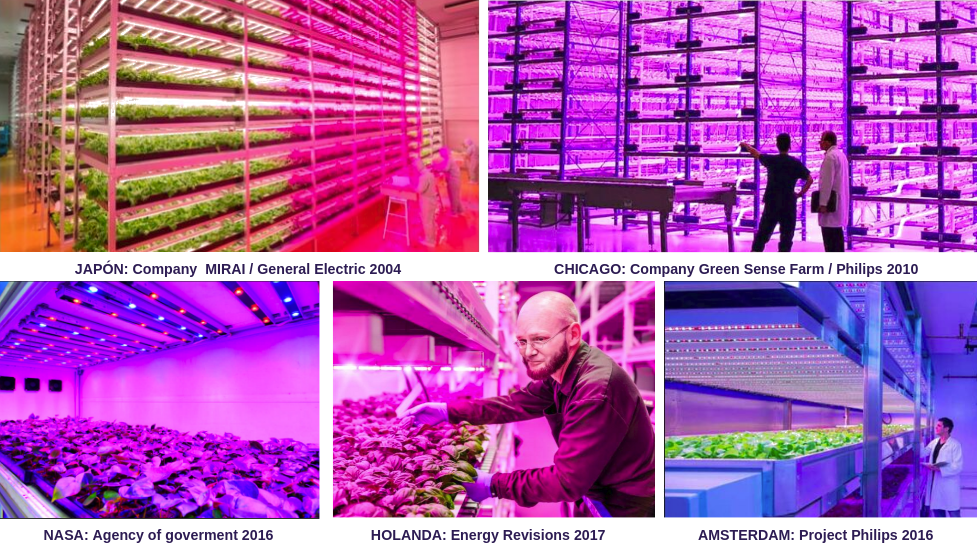
\includegraphics[width=16cm]{images/refMundialPAR.png}
   \caption{Status of technology: iot system for the monitoring and control of sources of artificial light applied to precision agriculture.\cite{diegojaviermenaamado2018} }
  \end{center}
\end{figure}
In Colombia, there is little scientific contribution in the field of lighting, colorimetry, radiometry and spectrometry for agriculture, however, it stands out a research by the researcher Lucia Atehortúa of the National University of Colombia, and this experimental research in the Francisco José de Caldas University District \textit{(UDFJC)}, which had as its general objective: ``Design, simulate and implement a modular IoT system for wireless monitoring and control of artificial light sources, capable of stimulating photosynthesis in plants".\cite{UNAL}
\\\\
Finally, we approach the reader of this article, with the experimental development of the prototype luminaire capable of storing metrics of spectrometric signatures of any plant genetics, considering that what was sought after the development of prototyping, was a similar system to that provided by Philips, with the connotation of using only free software tools.
%%----------------------------------------------------------
%%                MATERIAL AND METHODS
%%----------------------------------------------------------
\section{Materials and methods}

\subsection{Electronic design}
The reference project for the development of the proposed system was the luminaire device presented at the GreenTech in Amsterdam, since it was the only project that involved a database and metrics that could perfectly fit the scientific method of iteration that finally allows to conclude in the spectral plantprints, with which certain genetics have a better photosynthetic stimulus.
On the part of the calibration of the sensors involved and with the support of the laboratory of electrical and industrial tests of the National University of Colombia, several calibration measurements were generated to ensure the quality of the luminaire device. This laboratory has the necessary conditions to perform tests, since it is in conditions of total absence of light, isolated from noise and interference, which guarantees quality in the measurements.
Below are recommendations, materials and methods that were used to obtain the MVP or minimum viable prototype.
Selecting the right tools for any project visualizing requirements and scalability of a final product, leads to a considerable decrease in complexity. Given the functionalities of the system in general and analyzing the project as an application project, focused on precision agriculture, the technologies immersed in the system that allow determining the color composition with which each plant genetics would have a greater stimulus are briefly addressed. photosynthetic through its different stages or stages of life: germination, vegetation and flowering.

\subsection{Materials}
\subsubsection{LED technology for precision agriculture}
The LZP-00H100 LED emitter incorporates multiple critical wavelengths for proper plants growth. It went on sale at the end of 2016 and is capable of producing a photosynthetic photonic flux value \textit{(PPF)} of up to 106 umole/s; The primary lens of glass and other high quality materials, used in the package, are designed to offer a monumental robustness to challenging environment conditions with high temperature and humidity.
Main features:
\begin{itemize}
    \item Technology of specific purpose for applications oriented to precision agriculture.
    \item Mixture of photodiodes based on intelligent matrix positioning for high uniformity in wavelength radiation.
    \item Contains 4 channels, with fundamental wavelengths: blue \text(\SI{453}{\nano\metre}), deep red \SI{660}{\nano\metre}, far red \text(\SI{740}{\nano\metre}) and green \text(\SI{517}{\nano\metre}), in a single package.
    \item Lowest thermal resistance in the LED technology industry due to the spacing of the package, approximately \SI{0.5}{\degreeCelsius/\watt}.
    \item Power dissipation up to 70 W in a compact emitter footprint of 12 mm x 12 mm and maintenance projection after 20000 hours of operation.
\end{itemize}
For considerations of electronic design of the proposed system, some notes of the manufacturer were taken into account in order to consider accuracy in the radiation delivered by the device, the most important: maintaining a current flow of 700 mA; the accuracy is related to the bias of an estimate. The smaller the bias, the more accurate is an estimate. In that way the resulting typical wavelength would be in well-defined ranges.
\begin{itemize}
    \item Deep red: \SIrange{655}{670}{\nano\metre} peak wavelength.
    \item Far red: \SIrange{723}{745}{\nano\metre} maximum wavelength.
    \item Blue: \SIrange{453}{460}{\nano\metre} of dominant wavelength.
    \item Green: \SIrange{520}{530}{\nano\metre} of dominant wavelength.
\end{itemize}
In turn, the manufacturer recommends using lenses to increase the homogeneity of the irradiated light, focus or disperse according to the purpose to be considered, conditioning the typical pattern of space radiation of the glass provided by the LED.
\begin{figure}
 \begin{center}
  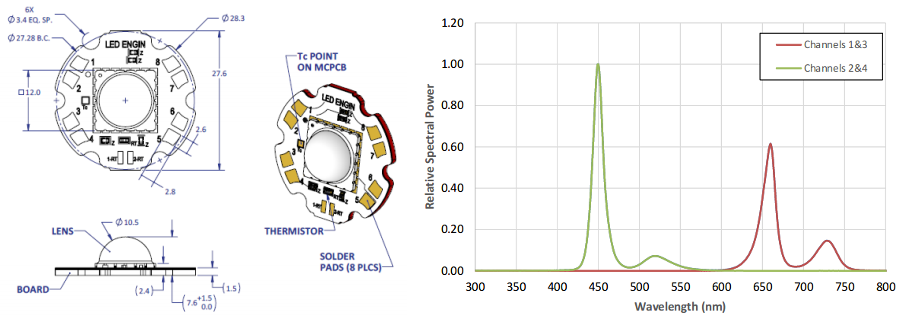
\includegraphics[width=16cm]{images/ledEngine.png}
   \caption{Presentation of Led LZP-00H100 and typical relative spectral power versus wavelength $@T_C = 25$~\si{\degreeCelsius}.\cite{ledEngine} }
  \end{center}
\end{figure}

\subsubsection{Lenses LLNF-4T11-H}
This lens family is combined with the LZP family of emitting diodes to ensure high and compact flow density. The lens maximizes the usable lumens in the target area. This lighting solution not only provides the range or distance required for wide lighting applications, but it does so with a beam of high uniformity, eliminating annoying reflections or shadows for plants. 
\begin{figure}
 \begin{center}
  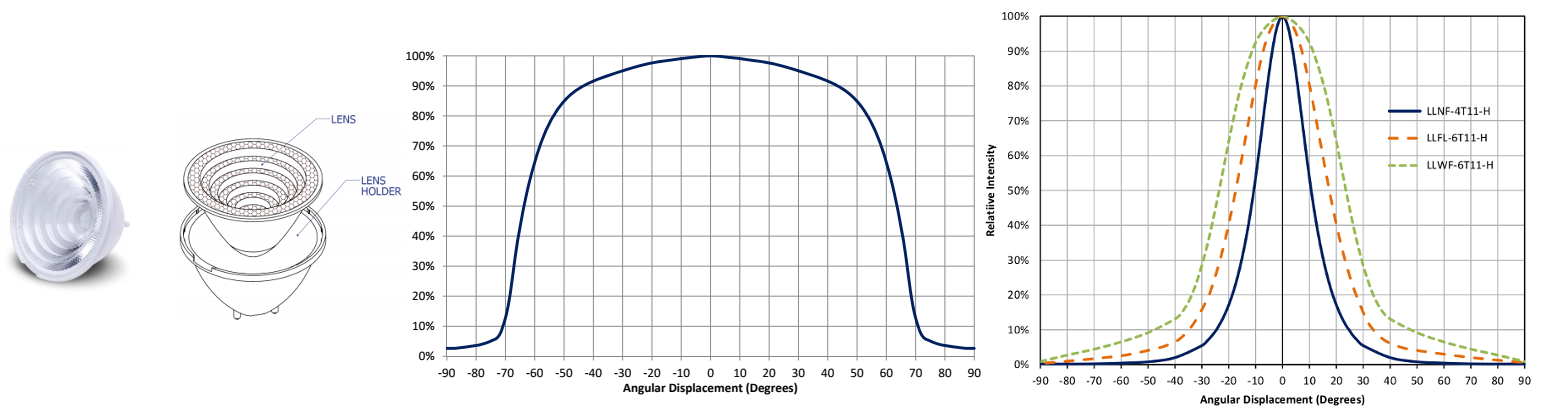
\includegraphics[width=16cm]{images/lente.png}
   \caption{Presentation of the lens LLNF-4T11-H. Typical pattern of space radiation of the LED and its correction with lenses. Angular displacement versus relative intensity.\cite{ledEngine} }
  \end{center}
\end{figure}
Main features of the lens:
\begin{itemize}
    \item Total internal reflection optics provide quality for well-controlled light beams.
    \item Provides excellent uniformity of color and amount of light.
    \item Its smooth light gradient eliminates hot spots and minimizes glare.
    \item ULMA rated optical grade PMMA lens material allows the use of high current conditions and supports high temperatures.
\end{itemize}
As can be seen in the previous graph, the LLNF-4T11-H lens allows concentrating the PAR radiation by correcting the angular displacement characteristic of the LZP-00H100 LED, it also provides homogeneity in the area to be irradiated and increases the number of lumens by 2.8 times provided by the LED device. The manufacturer ENGINE clarifies that: refrigeration systems must be used despite the fact that the device supports high temperatures.

\subsubsection{Heatsink Cooling H}
To reduce the effect or influence of the losses of the LED seen in the form of heat, it is decided to use an active cooling solution, that is, the union of a heatsink and a fan that allows the adequate thermal conditions to be guaranteed both for the proper functioning of LEDs as well as their associated lenses. Some of its most outstanding features:\cite{disipador} 
\begin{itemize}
    \item Life time leading in the industry.
    \item Silent fan operation.
    \item Commonly used in architectural, hanging, punctual and descending applications.
    \item Extremely efficient, consumption of \SI{0.18}{\watt}.
    \item Thermal power dissipation up to \SI{53}{\watt}.
\end{itemize}

\subsubsection{Power supply or electrical power}
Clearly the system in general requires a power supply that allows to energize the components of the power and control circuits necessary for the proper operation of the system in general. For this and thinking about allowing the system to manipulate several luminaire modules, it is decided to acquire the GWS500 source. Some of its most relevant characteristics are:\cite{fuenteDC}
\begin{itemize}
    \item High efficiency, up to $93\%$. Possible AC input of \SIrange{85}{264}{\volt}.
    \item It has an internal refrigeration system by convection of \SI{250}{\watt}.
    \item Default output voltage equivalent to \SI{36}{\volt}, but an adjustable range of \SIrange{32}{40}{\volt} can be used.
    \item Maximum current flow equivalent to \SI{7}{\ampere}.
    \item Maximum power to deliver equivalent to \SI{500}{\watt}.
\end{itemize}

\subsubsection{Light sensors}
\begin{figure}
 \begin{center}
  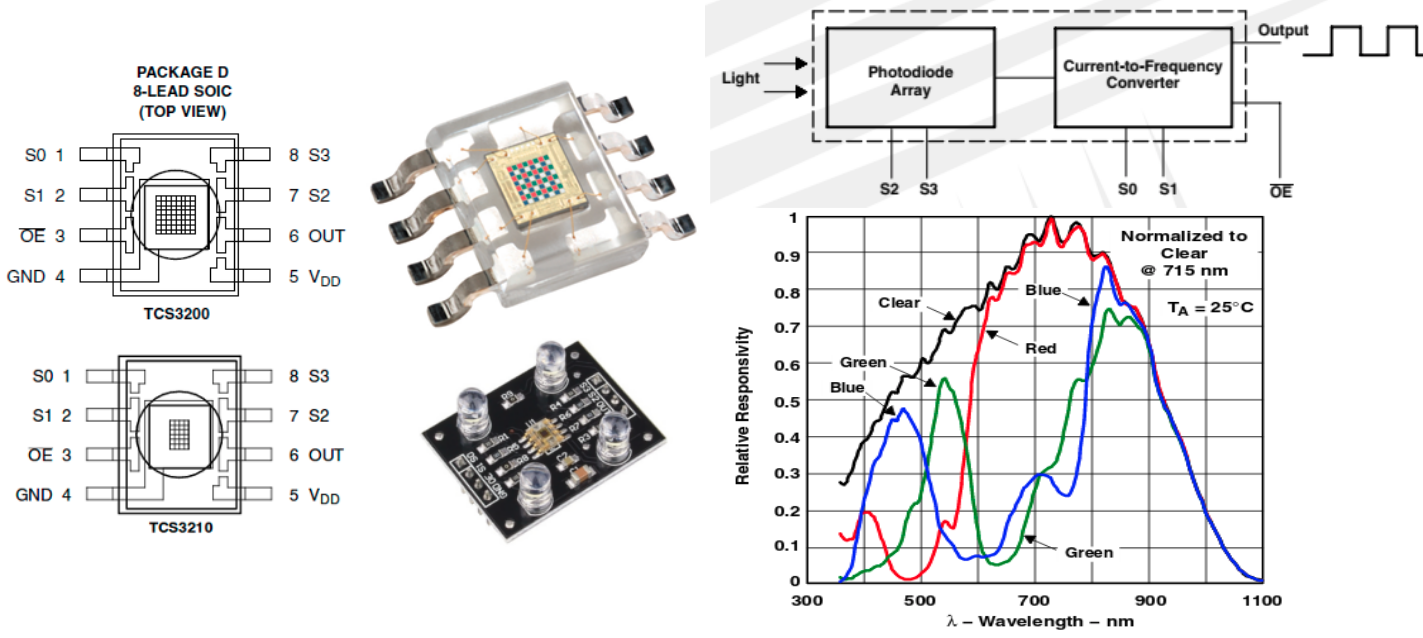
\includegraphics[width=16cm]{images/sensorLuzColor.png}
   \caption{Presentation of the TCS32xx sensors. Operation diagram and operation curves.\cite{tcs3200} } \end{center}
\end{figure}
Commonly called LTF \textit{(Light To Frequency)} devices, perform the functions of light detection, signal conditioning and analog-digital conversion in a monolithic package, capable of converting light to digital signals as a function of frequency. After evaluating the main transducers-light sensors that are commercialized in the market and bearing in mind the range of PAR radiation, programmable devices \textit{(plug and play)} are discarded given their high cost, in addition to not allowing flexibility in terms of electronic design . For this reason, the TCS32xx family of color sensors is considered to be involved in the system since they are easily adaptable sensors to development environments or microcontrollers and their technical specifications cover the needs of the project at low cost. The TCS32xx family of sensors transforms a color signal at a frequency with a polarization of \SIrange{2.7}{5.5}{\volt}, basically filtering the RGB data from a light source and converting it into a square signal with a certain frequency proportional to the composition of irradiated light. Some of its main characteristics by which they are implemented in the system are:
\begin{itemize}
    \item Typical non-linearity error of $2\%$ over \SI{50}{\kilo\hertz}.
    \item It is capable of capturing a broad spectrum of light (\SIrange{350}{900}{\nano\metre}) with high resolution.
    \item Supports temperatures between -40ºC and 70ºC.
    \item The TCS3210 sensor consists of a matrix of 4x6 photodiodes, 8 with red filters, 8 with green filters, 8 with blue filters and 8 without filters to make the general sweep of the spectrum.
    \item The TCS3200 sensor consists of a matrix of 8x8 photodiodes, 16 with red filters, 16 with green filters, 16 with blue filters and 16 without filters to make the general sweep of the spectrum.
\end{itemize}

\subsubsection{Raspberry Pi}
The Raspberry Pi mini-computer or low-cost single-board computer has the purpose in prototyping to be the main core to support the different control interfaces, data storage and the generation of PWM \textit{(Pulse-width modulation)} signals that allow adjust the time of switching for MOSFET technology devices that in turn allow to adjust the amount of power to be delivered to the luminaires. The technique used to generate these signals is extremely efficient: it does not use the CPU of the device and provides very stable pulses at \SI{100}{\hertz}. Although the Raspberry Pi includes two pins for the generation of PWM signals by hardware, it is decided to use the library blaster that generates this type of signals by software allowing that practically all the pins serve the purpose of generating PWM signals. This allows the system to be much more scalable since it can control several luminaires on the same system.
For greater understanding of this novel functionality, it is suggested to visit the official pi-blaster site directly in your repository hosted on github.\cite{pi-blaster}

\subsubsection{MOSFET Technology}
Bipolar transistors and MOSFETs handle a similar operating principle. Fundamentally, both types of transistors are controlled charge devices, which means that their output current is proportional to the charge established in the semiconductor by the control electrode. Theoretically, the switching speeds of bipolar and MOSFET devices are almost identical, determined by the time required for load carriers to travel through the semiconductor region. Typical values in power devices are approximately 20 to 200 picoseconds depending on the device.
The popularity and proliferation of MOSFET technology for digital and power applications is driven by two of its main advantages over bipolar junction transistors. One of these benefits is the ease of use of MOSFET devices in high frequency switching applications. MOSFET transistors are simpler to operate because their control electrode is isolated from the conductive silicon of the current, therefore, no direct current of ON is required. Once the MOSFET transistors are turned on, their drive current is practically zero; In addition, the ability to control load \textit{(energy)} and the storage time in MOSFET transistors is greatly reduced. As a result, MOSFET technology promises to use much simpler and more efficient drive circuits with significant economic benefits compared to bipolar devices.\cite{texasInstrument}
\subsubsection{Simulation of circuits and schematics}
The HEXFET power MOSFETs employed by International Rectifier use advanced processing techniques to achieve extremely low exposure resistance per area of silicon. This benefit, combined with the fast switching speed and reinforced device design whereby the HEXFET power MOSFETs are well known, provides the designer with an extremely efficient and reliable device to use in a wide variety of applications. The low thermal resistance and the low cost of the device contribute to its wide acceptance throughout the industry.
\begin{figure}
 \begin{center}
  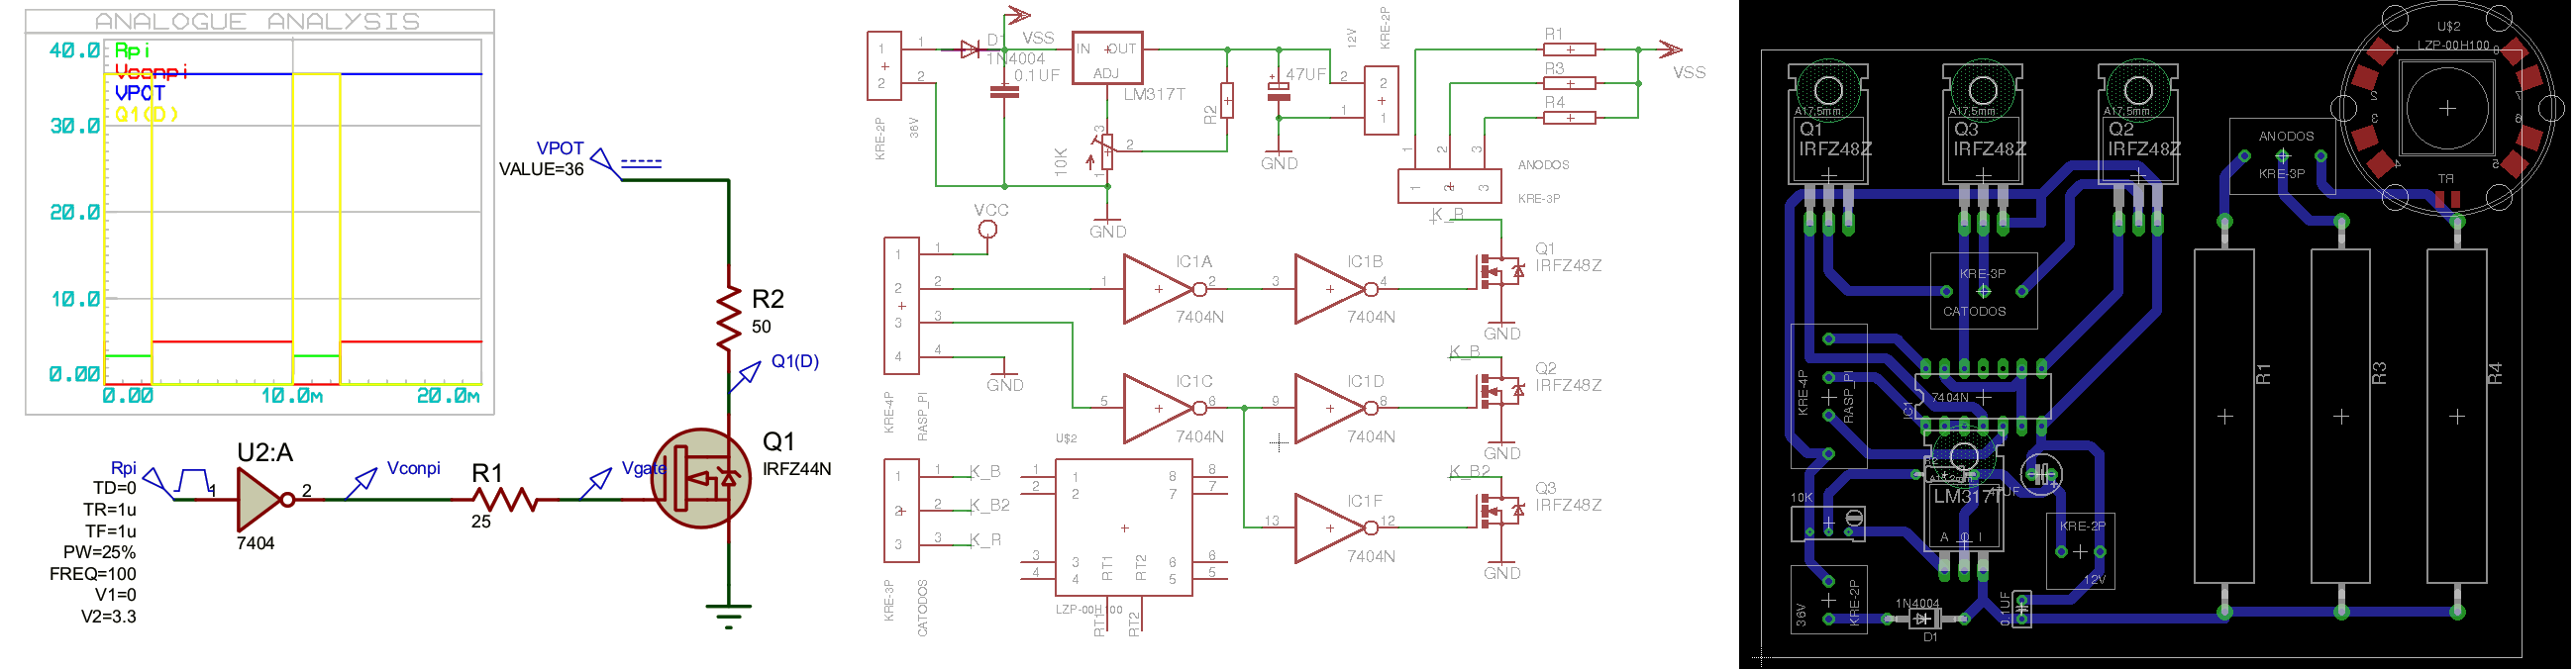
\includegraphics[width=16cm]{images/circuitoDriver.png}
   \caption{Simulation of the power circuit for a single channel of the 4 available by the LED. Schematic of the control and power circuit. MVP circuit PCB. \cite{wiki}} \end{center}
\end{figure}


%%----------------------------------------------------------
%%                RESULTS
%%----------------------------------------------------------
\section{Results}
\subsection{Research results}
The MVP developed is able to allow the end user full control of the power to be radiated in each of the light controllers, additionally allows you to create files as a logbook that hosts comments on the care of the plants, assigning them as relevant parameters together with the record of the date, time and composition of the color when making a new annotation. The integrity of the information provided by the LTF sensors of the system is attributed to its calibration thanks to the support of the laboratory of electrical and industrial tests of the National University of Colombia, where various measurements were generated to ensure the quality of the device. The laboratory has the necessary conditions to carry out tests, since it is isolated from noise and interference given that the site has conditions of total absence of light, which guarantees quality in the measurements. To do this, an SP-200 spectroradiometer was used to determine the wavelength radiated by the LED and in parallel the same measurements were made with our measurement system based on the TCS32xx sensor family. The SP-200 multifunction spectroradiometer has a versatile design that uses interchangeable accessories to allow the measurement of the spectral brightness, irradiance and luminous flux of a light source. The SP-200 detects which measurement head is connected and automatically changes the units of measurement and calibration files, making it the most versatile and cost-effective spectroradiometer available on the market. Its usability is enhanced by unique features that include an internal white point laser for radiance measurements that projects a circular image onto the device under test. This shows the user the region to be measured and eliminates the hassles of a viewer. The SP-200 also has the ability to simultaneously run up to 16 instruments on a single computer, enabling the capture of many test points for high-performance tasks.\cite{LABE}
\begin{figure}
 \begin{center}
  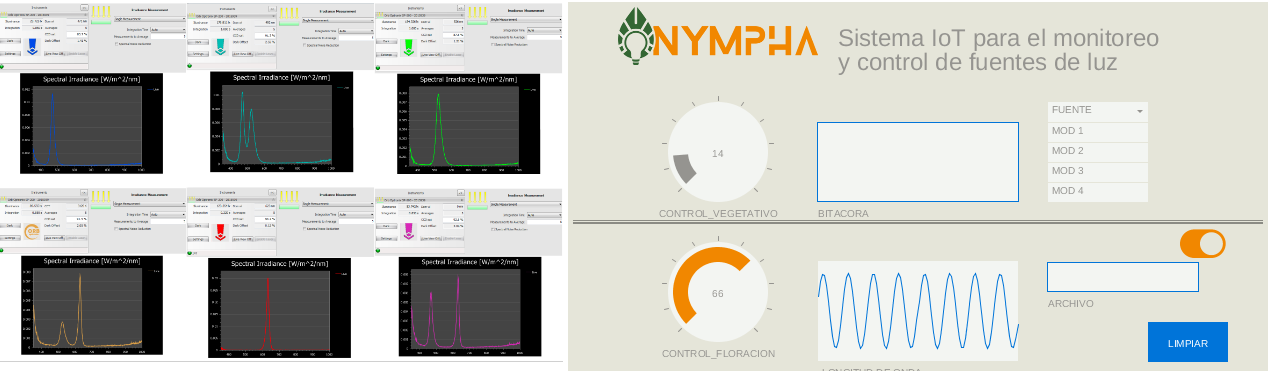
\includegraphics[width=16cm]{images/interface_data.png}
   \caption{Samples provided by the SP-200 spectroradiometer. User interface for the MVP. \cite{wiki}} \end{center}
\end{figure}
Basically, data were taken varying voltage intensity in power and distance, to achieve greater homogeneity in the data obtained, below are relevant data and graphics generated by the optical spectroscope. The software, in addition to indicating the measured wavelength, shows us the color trend, returning the curve obtained from the color to which it tends.
Given that the project was developed in a modular way, it is estimated that luminaire arrays will be designed in the near future, with not only four channels for color control \textit{(RGBW)} but twelve channels for color space compositions \textit{(HSV, HSL, CIE XYZ)} increasing the power capacity of the device and its color range in general.
\\\\\\
Once a frequency sweep is performed with the taking of different samples of the color in the photosynthetically active radiation spectrum, the response of the TCS32xx sensor family is established for each of the red, green, blue and unfiltered filters, with the In order to establish a mathematical model that allows to describe the most appropriate behavior of the sensor versus the spectroradiometer.
It was interesting to appreciate that the spectroradiometer interface highlighted curves with an emphasis on the color evaluated and for that reason something similar and dynamic was designed for the monitoring and control interface of the luminaire device.

\subsection{Research future}
Some researchers attending the IV International Congress of Research and Innovation of Engineering, Science and Food Technology IICTA 2018 where the MVP was presented, raised interests in the digital processing of microscopic images after the effect of different light compositions. \textit{(Chloroplasts and stomata in different plant genetics)} and a new power modulation technique for luminaires called pulse density modulation \textit{(Pulse-Density Modulation vs. the current pulse width modulation technique PWM)}. To learn more about this project, the reader is invited to visit the website \url{https://nympha.asharastudios.com/}
Acknowledgments to the Center for Scientific Research and Development CIDC for the economic support for this research.
%%----------------------------------------------------------
%%                CONCLUSIONS
%%----------------------------------------------------------
\section{Conclusions}
Optimization in agriculture is a challenge in which human survival, like that of other ecosystems, is involved. This project consisted in the use of specific light frequencies that allow specific photosynthetic processes in environments of total or partial absence of natural light. The artificial radiation processes are monitored through an interface that allows the control of frequencies, potnecy and time (photoperiod) to irradiate on the crop; It also allows you to store comments on the care of the plants in log mode, together with all the colorimetric data gathered from the sensors of the device, in real time. With this series of data, the luminaries are regulating their operation, feeding a database with millions of possible scenarios, finding the optimum for each of the situations and leading agriculture in any type of conditions to a sustainable and efficient productivity. Unlike devices in the market, the end user has full control of the system and can adjust its parameters to suit. The sensors used have a typical non-linearity error of 2\% and have been calibrated minutely in the LABE laboratory of optics and electrical tests of the National University of Colombia - Bogotá.
%%----------------------------------------------------------
%%                APPENDIXES
%%----------------------------------------------------------
% \appendix
% \section{First appendix}
% \section{Second appendix}
% Text of second appendix.
% %%
% %%   Add additional appendixes as you need.
% %%
% \section{Final appendix}
% Text of final appendix.
%%----------------------------------------------------------
%%                ACKNOWLEDGMENTS
%%----------------------------------------------------------
\section*{Acknowledgment}% <-- Please use \section*
We thank the research groups LASER (Automation Laboratory, embedded systems and robotics), GITUD (Telecommunications Research Group of the District University) and CIDC (Scientific Research and Development Center) thank you for the workspaces that they allowed the research to work out much better, in the same way I thank the human talent of the electrical testing laboratory of the National University of Colombia, because thanks to their support, many of the concerns about light and its understanding were solved.
%%----------------------------------------------------------
%%                REFERENCES
%%----------------------------------------------------------
\bibliography{biblio}%<-- bibliography's file (*.bib).
                  % This bibligraphy should be
                  % prepared by BibTeX.
                  % You can specify more *.bib files.
                  % ref.bib should be into the same
                  % directory of your source file
\bibliographystyle{plain}%<-- Style's file (*.bst).
%%----------------------------------------------------------
%%                BIOGRAPHIES
%%----------------------------------------------------------
\begin{biography}%
%%[{\includegraphics[width=1in]{photograph}}]%<-- author's photograph
                                            % Uncomment if
                                            % you need a photograph
{Diego Javier Mena Amado}% (Required)
Electronic engineer with experience in the development of digital products, passionate about science and technology. Promoter of free software and open design hardware. Electronic designer at Ashara Studios, specialist in developments about the internet of things.
\end{biography}
\begin{biography}%
%%[{\includegraphics[width=1in]{photograph}}]%<-- author's photograph
                                            % Uncomment if
                                            % you need a photograph
{Cesar Andrey Perdomo Charry}% (Required)
Biography of second author.
\end{biography}
%%
%%   Add more biographies as you need.
%%
\begin{biography}%
%%[{\includegraphics[width=1in]{photograph}}]%<-- author's photograph
                                            % Uncomment if
                                            % you need a photograph
{Luis Enrique Martin Santamaria}% (Required)
Electronic engineer, belonging to the GITUD research group of the Francisco José de Caldas University, with postgraduate studies and research in the areas of automatic and instrumentation.
\end{biography}
\end{document}
